\documentclass[10pt,letterpaper]{amspset}
\usepackage{fullpage}
\usepackage{gensymb}
\usepackage{graphicx}
\usepackage{tikz}
\graphicspath{ {./images/} }
\notag

% info for header block in upper right hand corner
\name{Brady Lamson}
\class{MATH 1120 SPRING 2021}
\assignment{Homework Part 1}
\duedate{Jan 31st}

\begin{document}

\problemlist{Unit Circle, Right Triangle and Trigonometric Functions Homework Assignment Part I:  

10.2 1—26, 28, 31—36, 40—44,  

10.3 1—28, 33, 34, 43—48, 55—61 }

I will be repeatedly referencing the "Important Points of the Unit Circle" figure and a table of sine and cosine values. Both will be included in the reference section of this assignment. \bigskip


In Exercises 1-20, find the exact value of the cosine and sine of the given angle.

\begin{problem}[1.]
$\theta = 0$
\end{problem}

\begin{solution}
It is important to note that cosine and sine represent the x and y coordinates respectively. This makes this starting problem incredibly easy. 0, be it in degrees or radians, lands us right at the beginning. This gives us the following answers.
\[\boxed{cos(0) = 1}\]
\[\boxed{sin(0) = 0}\]

\end{solution}


\begin{problem}[2.]
$\theta = \frac{\pi}{4}$
\end{problem}

\begin{solution}

\begin{center}
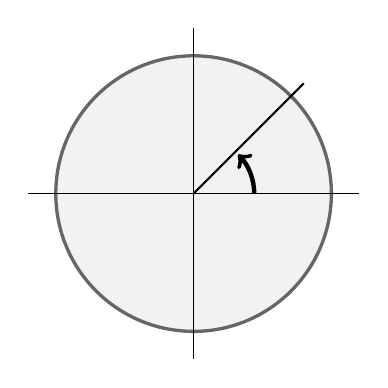
\begin{tikzpicture}[scale=0.7]
        \filldraw[color=black!60, fill=black!5, very thick](0,0) circle (2.5);
        \draw (-3,0) -- (3,0);
        \draw (0,3) -- (0,-3);
        \draw [thick ] (0,0) -- (2,2);
        \draw[ultra thick, ->] (1.1,0) arc (0:45:1);
    \end{tikzpicture}
\end{center}


\end{solution}






\pagebreak
\centering \textbf{References}     


Figure 1.
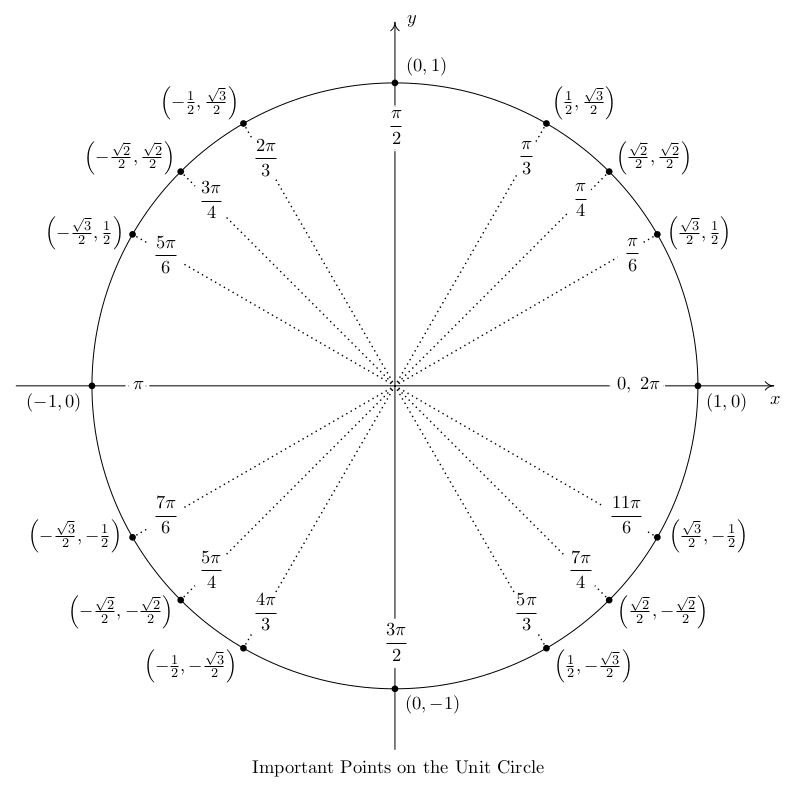
\includegraphics[width=6in,scale=1.0]{images/unit_circle.png}

Figure 2.
\begin{center}
\begin{tabular}{ |c|c|c|c| } 
 \hline
  $\theta$(degrees) & $\theta$(radians) & cos($\theta$) & sin ($\theta$) \\ [1.0ex] 
 \hline\hline
 0\degree & 0 & 1 & 0 \\[+3mm] 
 $30\degree$ & $\frac{\pi}{2}$ & $\frac{\sqrt{2}}{2}$ & $\frac{1}{2}$ \\[+3mm] 
 $45\degree$ & $\frac{\pi}{4}$ & $\frac{\sqrt{2}}{2}$ & $\frac{\sqrt{2}}{2}$\\[+3mm]
 $60\degree$ & $\frac{\pi}{3}$ & $\frac{1}{2}$ & $\frac{\sqrt{3}}{2}$\\[+3mm]
 $90\degree$ & $\frac{\pi}{2}$ & 0 & 1 \\
 \hline
\end{tabular}
\end{center}
\end{document}
